\documentclass{sigchi}

% Use this section to set the ACM copyright statement (e.g. for
% preprints).  Consult the conference website for the camera-ready
% copyright statement.


%%% Local Variables:
\newcommand{\xray}{XRAY\xspace}
%%% mode: latex
%%% TeX-master: t
%%% End:

% Copyright
\CopyrightYear{2016}
%\setcopyright{acmcopyright}
\setcopyright{acmlicensed}
%\setcopyright{rightsretained}
%\setcopyright{usgov}
%\setcopyright{usgovmixed}
%\setcopyright{cagov}
%\setcopyright{cagovmixed}
% DOI
\doi{http://dx.doi.org/10.475/123_4}
% ISBN
\isbn{123-4567-24-567/08/06}
%Conference
\conferenceinfo{CHI'16,}{May 07--12, 2016, San Jose, CA, USA}
%Price
\acmPrice{\$15.00}

% Use this command to override the default ACM copyright statement
% (e.g. for preprints).  Consult the conference website for the
% camera-ready copyright statement.

%% HOW TO OVERRIDE THE DEFAULT COPYRIGHT STRIP --
%% Please note you need to make sure the copy for your specific
%% license is used here!
% \toappear{
% Permission to make digital or hard copies of all or part of this work
% for personal or classroom use is granted without fee provided that
% copies are not made or distributed for profit or commercial advantage
% and that copies bear this notice and the full citation on the first
% page. Copyrights for components of this work owned by others than ACM
% must be honored. Abstracting with credit is permitted. To copy
% otherwise, or republish, to post on servers or to redistribute to
% lists, requires prior specific permission and/or a fee. Request
% permissions from \href{mailto:Permissions@acm.org}{Permissions@acm.org}. \\
% \emph{CHI '16},  May 07--12, 2016, San Jose, CA, USA \\
% ACM xxx-x-xxxx-xxxx-x/xx/xx\ldots \$15.00 \\
% DOI: \url{http://dx.doi.org/xx.xxxx/xxxxxxx.xxxxxxx}
% }

% Arabic page numbers for submission.  Remove this line to eliminate
% page numbers for the camera ready copy
% \pagenumbering{arabic}

% Load basic packages
\usepackage{balance}       % to better equalize the last page
\usepackage{graphics}      % for EPS, load graphicx instead 
\usepackage[T1]{fontenc}   % for umlauts and other diaeresis
\usepackage{txfonts}
\usepackage{mathptmx}
\usepackage[pdflang={en-US},pdftex]{hyperref}
\usepackage{color}
\usepackage{booktabs}
\usepackage{textcomp}
\usepackage{xspace} % naomi


% Some optional stuff you might like/need.
\usepackage{microtype}        % Improved Tracking and Kerning
% \usepackage[all]{hypcap}    % Fixes bug in hyperref caption linking
\usepackage{ccicons}          % Cite your images correctly!
% \usepackage[utf8]{inputenc} % for a UTF8 editor only

% If you want to use todo notes, marginpars etc. during creation of
% your draft document, you have to enable the "chi_draft" option for
% the document class. To do this, change the very first line to:
% "\documentclass[chi_draft]{sigchi}". You can then place todo notes
% by using the "\todo{...}"  command. Make sure to disable the draft
% option again before submitting your final document.
\usepackage{todonotes} % naomi
\usepackage[normalem]{ulem} % also naomi

% Paper metadata (use plain text, for PDF inclusion and later
% re-using, if desired).  Use \emtpyauthor when submitting for review
% so you remain anonymous.

\def\plaintitle{XRAY: Inspector Tools For Designers}
\def\plainauthor{First Author, Second Author, Third Author,
  Fourth Author, Fifth Author, Sixth Author}
\def\emptyauthor{}
\def\plainkeywords{Web design; design systems; inspector tools; experimentation; human factors; developers; designers. 
}
\def\plaingeneralterms{Documentation, Standardization}

% llt: Define a global style for URLs, rather that the default one
\makeatletter
\def\url@leostyle{%
  \@ifundefined{selectfont}{
    \def\UrlFont{\sf}
  }{
    \def\UrlFont{\small\bf\ttfamily}
  }}
\makeatother
\urlstyle{leo}

% To make various LaTeX processors do the right thing with page size.
\def\pprw{8.5in}
\def\pprh{11in}
\special{papersize=\pprw,\pprh}
\setlength{\paperwidth}{\pprw}
\setlength{\paperheight}{\pprh}
\setlength{\pdfpagewidth}{\pprw}
\setlength{\pdfpageheight}{\pprh}

% Make sure hyperref comes last of your loaded packages, to give it a
% fighting chance of not being over-written, since its job is to
% redefine many LaTeX commands.
\definecolor{linkColor}{RGB}{6,125,233}
\hypersetup{%
  pdftitle={\plaintitle},
% Use \plainauthor for final version.
%  pdfauthor={\plainauthor},
  pdfauthor={\emptyauthor},
  pdfkeywords={\plainkeywords},
  pdfdisplaydoctitle=true, % For Accessibility
  bookmarksnumbered,
  pdfstartview={FitH},
  colorlinks,
  citecolor=black,
  filecolor=black,
  linkcolor=black,
  urlcolor=linkColor,
  breaklinks=true,
  hypertexnames=false
}

% create a shortcut to typeset table headings
% \newcommand\tabhead[1]{\small\textbf{#1}}

% End of preamble. Here it comes the document.
\begin{document}

\title{\plaintitle}

\numberofauthors{3}
\author{%
  \alignauthor{Leave Authors Anonymous\\
    \affaddr{for Submission}\\
    \affaddr{City, Country}\\
    \email{e-mail address}}\\
  \alignauthor{Leave Authors Anonymous\\
    \affaddr{for Submission}\\
    \affaddr{City, Country}\\
    \email{e-mail address}}\\
  \alignauthor{Leave Authors Anonymous\\
    \affaddr{for Submission}\\
    \affaddr{City, Country}\\
    \email{e-mail address}}\\
}

\maketitle

\begin{abstract}
Examples are widely used by both designers and developers in the creation of websites. Numerous tools have been created to facilitate developers' borrowing of code from live websites and design examples. However, little work has been done to improve the experience of designers working on partially-developed or live sites. This paper introduces \xray, inspector tools for designers (Figure~\ref{fig:xray_screenshot}). Unlike traditional inspector tools, \xray allows the designer to adjust fonts, colors, margins, and padding without ever needing to look at HTML or CSS, making this technical, traditionally code-based task more approachable for designers. \xray promotes the use of design systems by only suggesting styling options that exist in the current design system and highlighting where current aesthetics violate the design system. \xray also improves designer-developer communication by allowing people in different locations are able to make live edits to a website collaboratively. \xray allows users to export a document with all changes at the end of their session. 
Moreover, a 12 person user study with novices and a 12-person user study with professional designers showed that people were xx\% more efficient, yy\% more successful, and experimented more by using zz\% more styles when they used \xray, than when they used the standard industry tools. 
\end{abstract}


% Running questions/comments: 
% are we calling users: users? people? designers? 
% I know every other sentence starts with the word "XRAY" and I will eventually get around to fixing it

\category{H.5.m.}{Information Interfaces and Presentation
  (e.g. HCI)}{Miscellaneous} \category{See
  \url{http://acm.org/about/class/1998/} for the full list of ACM
  classifiers. This section is required.}{}{}

\keywords{\plainkeywords}
\section{Introduction}


\begin{figure}
    \centering
    
\includegraphics[width=\columnwidth]{figures/windows_lunch.jpg}
    \caption{A screenshot of the \xray user interface and the menu for [fonts? colors? margin/padding?]}  
    \label{fig:xray_screenshot}
\end{figure}

Both programmers and web designers look at websites for design inspiration and at snippets of code for guidance. Researchers and industry professionals have made developers tools to enable these programmers and designers to learn more from these examples. However, many of these tools are geared towards those who are comfortable with code. 

While there are some designers who can write code, and there are some developers who understand design, most professionals in industry specialize. Creating an app, website, or any product with a UI becomes a collaborative and iterative process. For example, if a company was preparing to launch a new website, the designer would create a mockup of how the product should look and send it to the developer. The developer would code it, and send it back to the designer. No first draft is flawless and the designer now needs to communicate the mistakes to the developer. 

Some designers will meet with the developers, sitting next to them and explaining what needs to be changed. However, that is very time-consuming for both the developer and designer. Other designers might send an email with a checklist of what needs to be fixed, but matching the block of test to the website gets confusing very quickly. In reality, it is most common for the developer to ``redline'' by marking up a screenshot of the website using tools like Sketch or InVision, such as in Figure~\ref{fig:markup_redline_website} as taken from Moore's 2017 Medium article \cite{digital_whiteboards_moore_medium_2017}. 

\begin{figure}
    \centering
    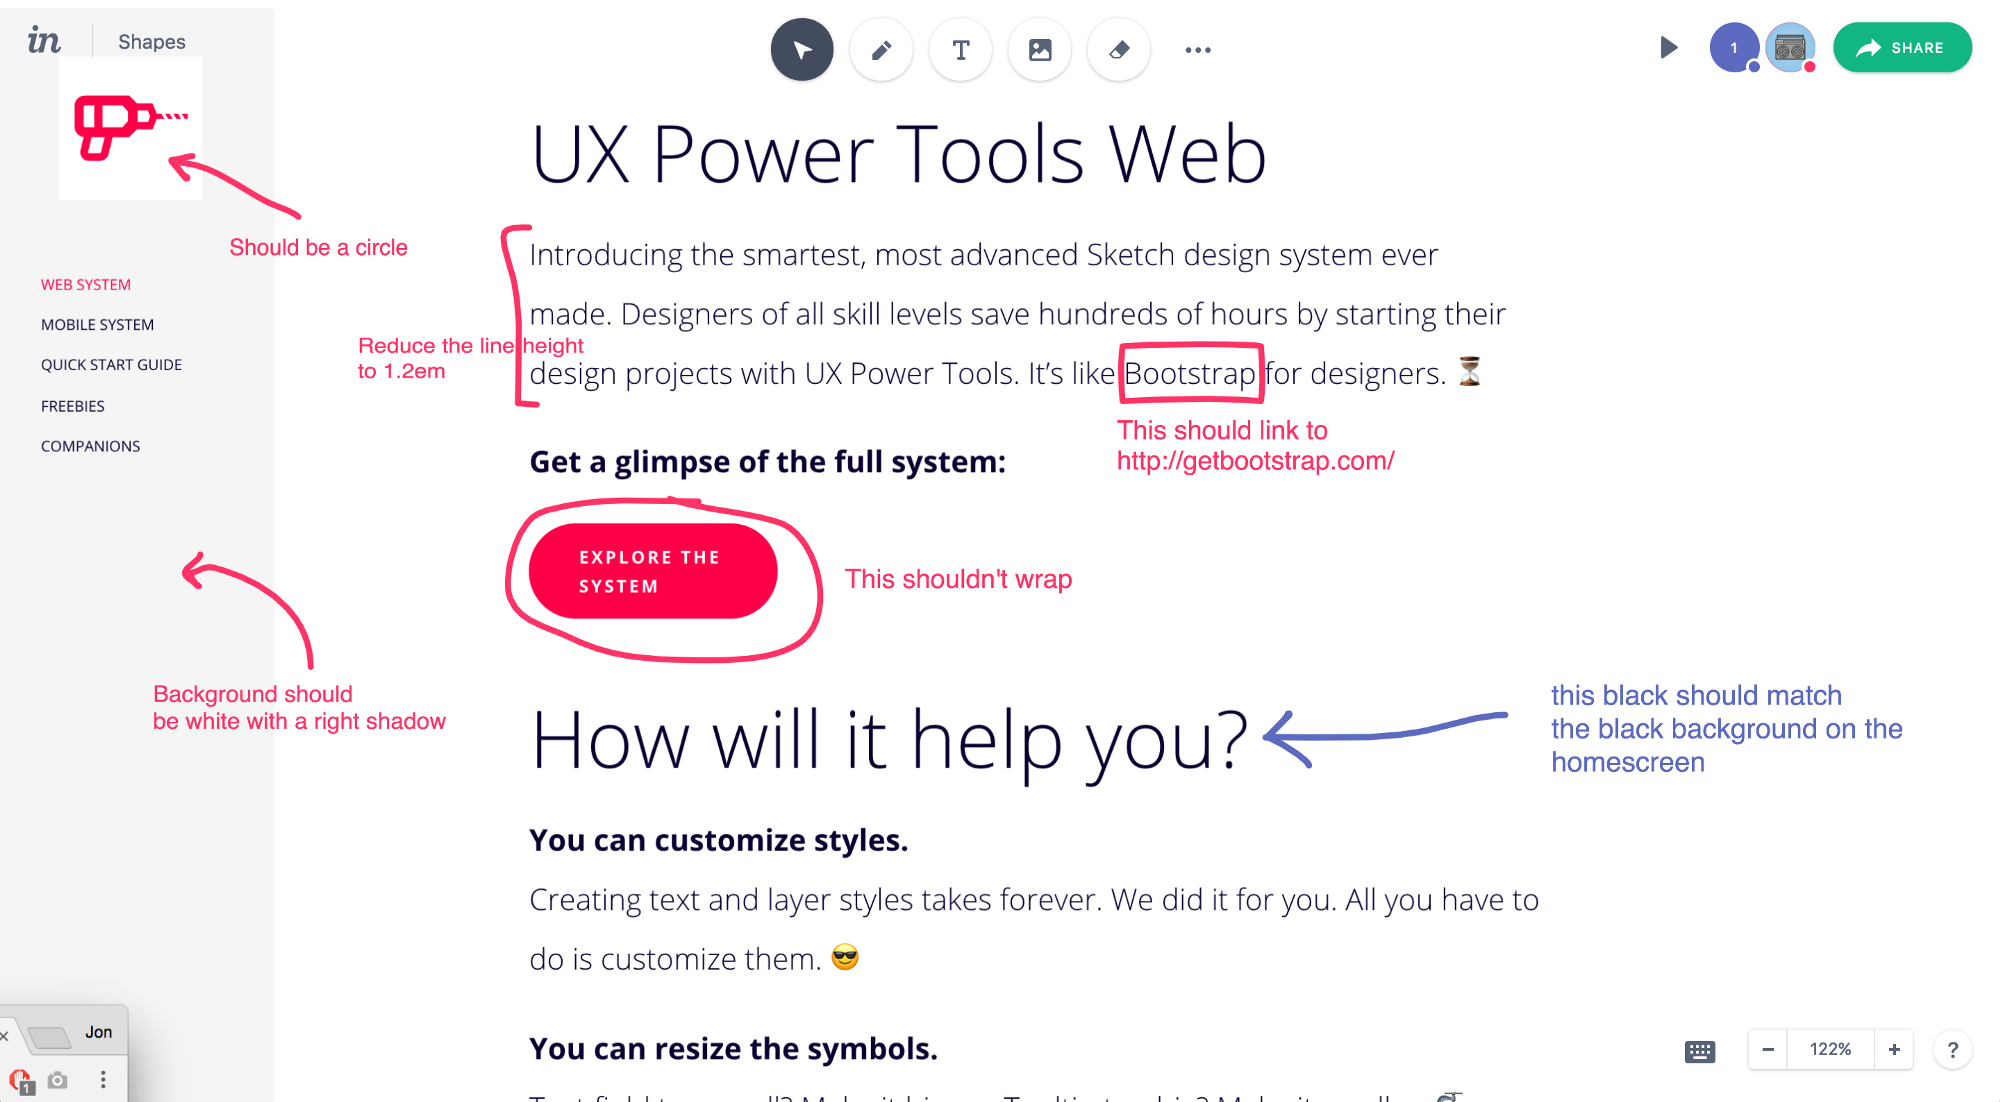
\includegraphics[width=\columnwidth]{figures/screenshot_redline_found_google.png}
    \caption{Example of a ``redline'' or markup of website that a designer might send to a developer}
    % https://medium.com/ux-power-tools/invision-freehand-digital-whiteboarding-bf83639c1184
    % \cite{digital_whiteboards_moore_medium_2017
    \label{fig:markup_redline_website}
\end{figure}

The ability to write comments on a screen simplifies the revision process. Instead of writing an essay for each bullet point (``the icon of a drill on the top left of the home page should be enclosed by a circle instead of a square''), the designer can draw an arrow to the icon they are dissatisfied with and write ``should be a circle.'' 

However, when it comes to colors, padding, and other sizing issues, detail is key. Instead of saying ``this black should match the black background on the homescreen'', why not just tell the developer the hexcode of the color it should be? Additionally, prior work shows the benefits of experimentation, yet writing notes on screenshots does not really provide that opporunity. Ideally, when the designer notices that the line height is too large, they would have the opportunity to see what the page would look like with 1.1em, 1.2em, and 1.3em before telling the developer which one is best. 

% of colors, fonts, spacing rules, and a library of pre-built widgets used in one website, app, or company.  
Currently, the developers are gatekeepers: they control the design and aesthetics of a finished product even though they do not have the knowledge or training that a designer does. The designers are in the uncomfortable position of knowing exactly how the final product should look, but are unable to create it themselves. 

(fix this next paragraph \#whatadisaster)


In order to provide designers with more control, many companies are creating design systems. Just as developers use a style guide in order to have a standardized way of doing things, designers create design systems. In order to create a brand image for customers [fix English], companies pick a color palette and a set of fonts to use on their websites, emails, advertising campaign, and app [cite]. Design systems evolved from style guides. In a 2017 Medium article, Couldwell defined explained his company's design system contains a set of text styles, color palettes, widgets, templates, and patterns \cite{design_system_at_plasma_couldwell_medium_2017}. 

% One key part of design is consistency [cite some papers].

When developers and designers face seemingly small questions like ``How should we format the time/date/currency?'' or ``What kind of color/typeface/button should I use?'' or ``Should this be sentence case or title case?'', the design system can evolve to hold these answers \cite{what_is_design_system_couldwell_medium_2017}. Often a [file type] or [photoshop file], the design system can contain images of what these fonts, colors, and widgets look like, as well as the code to make them. This prevents developers from making the same buttons over and over for each website, and ensures that the color, shadow, and animated reaction for each click or hover over the button will be exactly the same \cite{what_is_design_system_couldwell_medium_2017}. 

Although the use of design systems is spreading rapidly in industry, we are not aware of any research regarding the creation or use of them. Companies including [list them] are currently using them; some began creating their design system as early as [year]. 

In order to 1. improve the experience of web designers, 2. improve their collaboration with developers, and 3. to promote the use of design systems, we built \xray (Figure~\ref{fig:xray_screenshot}), design-oriented inspector tools for developers. Unlike traditional inspector tools, \xray allows the designer to adjust fonts, colors, margins, and padding without ever needing to look at HTML or CSS, making this technical, traditionally code-based task more approachable for designers. 

% ALSO, (A. Allows designer to work in same medium as developers (as opposed to graphical tools like sketch), and B. Allows designer to better understand how websites are made/visualize element style and positioning i. Margin v. padding, etc)

\xray makes the following contributions: 

\begin{itemize}
    \item A novel set of inspector tools, designed for those who do not need to understand how HTML and CSS work. \xray allows users to adjust fonts, colors, margins, and padding on live sites without ever looking at any code. 
    
    \item \xray focuses on design systems. By only suggesting choices that are in the current design system, it helps novice designers be consistent. \xray provides the option to override these design guidelines, allowing users to expand the design system by adding new rules. When users redefine an aspect of their design system, \xray automates consistency, letting the changes percolate through not only the current page but the entire website, persisting even after page reloads. \xray highlights where a site breaks from the design systems, letting users quickly identify possible issues. 
    
    \item Designer-developer communication is improved because people in different locations are able to make live edits to a website collaboratively. At the end of a session, designers can export a document with all of their final changes noted in HTML and CSS to give to the developer.  
    
    \item A within-subject evaluation of \xray in comparison to the industry standard of using Sketch(c) to note flaws in a website. We had a total of 24 partcipants, half of whom were design professionals with a minimum of five years' experience, and half of whom were design students at our university. Our results showed that people were xx\% more efficient, yy\% more successful, and experimented more by using zz\% more styles when they used \xray, than when they used the standard industry tools.
\end{itemize}


\section{Related Works}
% \\important: transferring CSS from one site to another (get that in related works!!) 

% \\there aren’t research papers about design systems (site that airbnb paper, large companies that have these design systems) (we need this common vocabulary/language/common ground to facilitate designer/developer communication. Take what exists in the code and get it into figma/other graphic editor environments. #unification) 

Researchers are well aware that looking at examples to find inspiration is a key part of the creative process for both designers [cite things] and developers [cite things]. Recent work has considered the use of design galleries to assist in web design \cite{dtour_Ritchie_UIST_2011, interactive_example_galleries_Lee_CHI_2010} and in animation \cite{designGalleries_mitsubishi_Marks_SIGGRAPH_1997}. Webzeitgeist and other research projects have delved into the world of design-mining websites \cite{Webzeitgeist_Kumar_CHI_2013, learning_on_web_design_Satyanarayan_CHI_2012} and mobile apps \cite{mining_mobile_applications_alharbi_phdthesis_2016}. Other researchers have focused on smaller-scale projects. For instance, retargeting a design to a new size or aspect ratio \cite{learning_layouts_single_page_design_o_donovan_IEEE_2014}, or reformatting text \cite{review_automatic_docu_formatting_Hurst_DocEng_2009}, or both text and images \cite{probabilistic_auto_document_composition_Damera_Venkata_DocEng_2011}. Others have focused on getting one document to be easily readable on different screen sizes and shapes \cite{adaptiveGridBasedLayout_Jacobs_SIGGRAPH_2003}.

Other works have focused on helping developers use and understand snippets of code from other sites [cite]. Work on transferring CSS from one site to other has proven helpful for both developers and designers [cite] [this might be a whole paragraph], and other projects have focused on helping non-programmers coding  \cite{dinah_non_programmers_coding_Gross_CHI_2011}. (is the sketching thing related? \cite{retrieving_websites_with_sketches_example_based_design_hashimoto_igarashi_EUROGRAPHICS_EWSBIM_2005}). (Linked Editing (https://dl.acm.org/citation.cfm?id=1034566) This might not fit here, but it should give us language when we talk about editing multiple instances at the same time.).  

but often leans on the assumption that designers can code and coders can design. That isn’t what reality is like: many people in industry can either code OR design. 

Moreover, there is very little work being done with design systems. (already said what they are) touch again on why they are important/what the benefits are. 


% \begin{itemize}
%     \item Looking at other examples = important for both designers and developers. 
%     Geared towards designers: Research has included design galleries and the gathering of designs (whole pages) or pieces of pages. Geared towards developers: using snippets of code from/understanding live sites. For BOTH designers and developers, there has been research about transferring CSS from one site to other. 

% There are also tools and studies on However, there is very little work being done to create web dev related tools for developers. A lot of research seems to be focusing on 

%     \item 

% \end{itemize}

% \begin{itemize}
%     \item Use of examples in design galleries
%     \item Patterns found after design mining
%     \item Actual design patterns for websites
%     \item Using snippets of code from/understanding live sites
%     \item Other tools for developers
%     \item Transferring CSS from one site to other
%     \item But there are few tools for designers (list)
%     \item Sketching tools \cite{retrieving_websites_with_sketches_example_based_design_hashimoto_igarashi_EUROGRAPHICS_EWSBIM_2005}
%     \item Helping non-programmers select code \cite{dinah_non_programmers_coding_Gross_CHI_2011}
%     \item Overall, designers have it really rough, and a lot of research seems to be focusing on designers who can code and coders who can design. That isn’t what reality is like: many people in industry can either code OR design. 
%     \item Why are design systems important? What’s their benefit? [Maybe this belongs in the intro, but we’ll want to have a reference].
%     \item Linked Editing (https://dl.acm.org/citation.cfm?id=1034566) This might not fit here, but it should give us language when we talk about editing multiple instances at the same time.
% \end{itemize}
% 

\section{Interface and Features of XRAY}
First: overall things. Is a chrome plugin? Can use on any website. 

Lets you adjust and change: 


Fonts (family, weight), colors, margin, padding

Automatically downloads Google fonts to make them available on the website. This is often a very tedious task that requires the designer to either install the fonts locally or have access to the code.
You can copy and paste styles from one element to the next 


Doesn’t need to be same page

Get an instant preview of those changes

Can toggle on and off individual styles 

This means several sources can be pasted into same element (only really important because Web Crystal focuses a lot on this).

Lets you download your changes (to give to developer) (final visual changelog)

Developer now knows exactly what to do

Which will result in less work for designer as well

Whitespace is broken down into padding and margin. Normal redline documents only show spacing, but not whether it is margin or padding.

Changes persist across page reloads 

Changes to symbols persist not only across page reloads but also across the whole website, even on different pages. 

Can have changes permeate through a whole page

Many of these things help you see the design system (trees v. forest) 

Visualize website structure. Margin \& Padding is invisible and it is often difficult to know how whitespace is assigned. This tool colors the whitespace to show the structure.

Gives a live audit of the design system to show elements that diverge. 

I have implemented this yet, but we could make this collaborative, so two people could make live edits to a website collaboratively. It’s not very practical I don’t think, but it is shiny.

A corollary to this is instead of exporting a file to give to developers, the designer can just share the session with a developer and they can have a live editor of the changes.


\section{User Study}
\subsection{Participants}
12 students
12 professionals

\subsection{Tasks}
A, B, C (or) A, B

\subsection{Procedure}
And fill in this section too

\subsection{Results}
And put some graphs and stats and stuff in here

\section{Discussion (hard to write until we have results)}
Implications of results to science
Implications of results to practice 
Limitations
Further research 


\section{Conclusion}
Discuss benefits...

Discuss harm/risks/dangers/drawbacks...

Discuss future work/room to grow...







% BALANCE COLUMNS
\balance{}

% REFERENCES FORMAT
% References must be the same font size as other body text.
% \nocite{*}
\bibliographystyle{SIGCHI-Reference-Format}
\bibliography{xray}

\end{document}

